\documentclass{article}
\usepackage[utf8]{inputenc}
\usepackage[margin=1in]{geometry}
\usepackage{graphicx}
\usepackage{natbib}
\usepackage{enumitem}
\usepackage{array}
\usepackage{gensymb}
\usepackage{indentfirst}
\graphicspath{ {Images/} }
\usepackage{float}
\usepackage[table,xcdraw]{xcolor}
\usepackage{amsmath}

\title{Physics 111A Fall 2016- Lab 7\\
Op Amps II}
\author{Joshua Levy\\Lab Partner: Alex Chuang}
\date{October 16th, 2016}

\begin{document}

\maketitle

\section{Lab Write Up}
    %1
    \subsection{Negative Impedance Converter (NIC)}
    \begin{figure}[H]
        \centering
        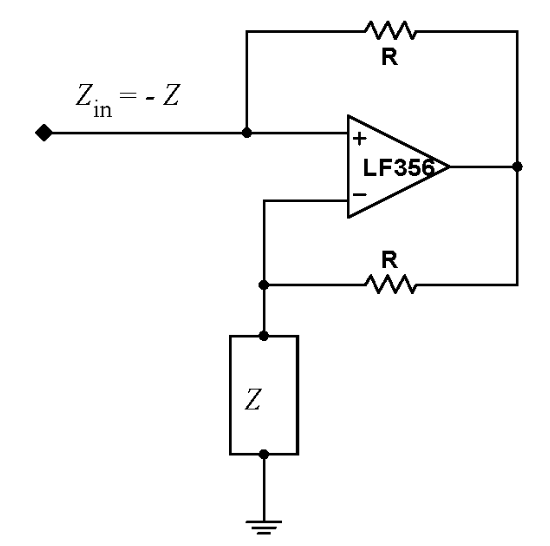
\includegraphics[scale = 0.6]{1.png}
        \caption{Negative Impedance Converter \cite{lab7}}
        \label{fig:my_label}
    \end{figure}
    We built the circuit above and measured one of the resistors (R) to be 2.272 $\Omega$ and the other to be 2.273 $\Omega$. We checked to see whether the 10k resistor is behaving properly by connecting the meters (see figure below) to point A and measuring the voltage drop across the 10k resistor and seeing if the current passing through the resistor and the voltage drop were both positive:
    \begin{figure}[H]
        \centering
        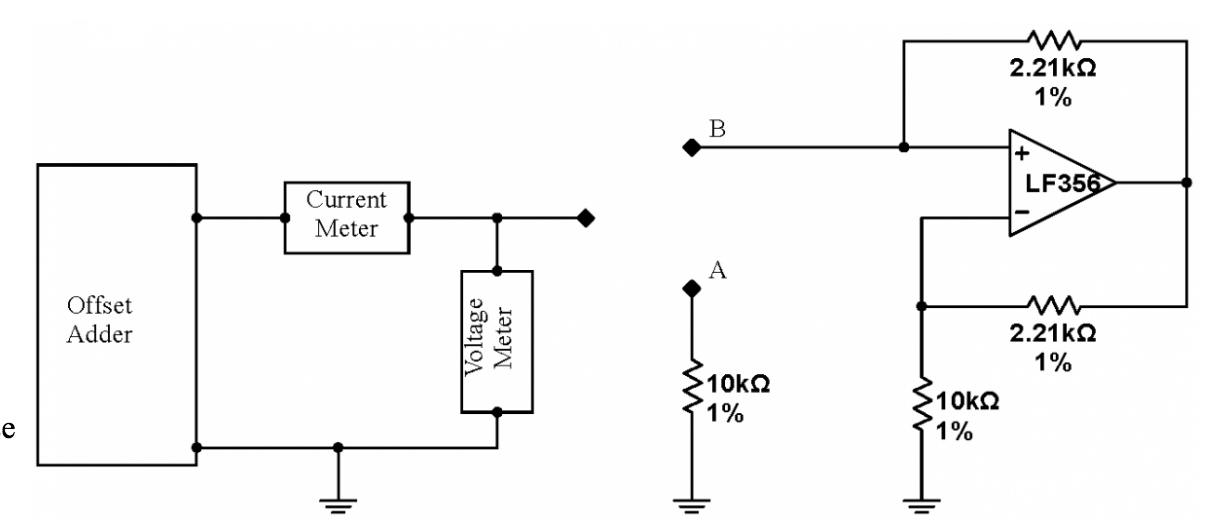
\includegraphics[scale = 0.6]{1a.png}
        \caption{Offset Adder Hooked Up to the NIC in Question  \cite{lab7}}
        \label{fig:my_label}
    \end{figure}
    Varying the offset values through different and negative values, and we noticed that the voltage drop across the 10k resistor had the same sign as the current passing through the 10k resistor. Thus, the 10k resistor behaves appropriately.\\\indent After connecting the meters to point B, we varied the offset adder voltage and measured the current. We noticed through application of the Op Amp Golden Rules that the offset adder voltage was the same voltage dropped across the 10k resistor. We measured the following values for the offset adder voltage and the current through the 10k resistor:
        \begin{table}[H]
        \centering
        \caption{Voltage and currents across the 10k resistor hooked up to the NIC}
        \label{my-label}
        \begin{tabular}{ll}
        \textbf{V (mV)} & \textbf{Current I (mA)} \\ \hline
        10 & -0.0043 \\
        1000 & -0.101 \\
        2000 & -0.1967 \\
        4020 & -0.394 \\
        9290 & -0.921
        \end{tabular}
        \end{table}
    This data plotted with current vs. offset adder voltage yields:
        \begin{figure}[H]
            \centering
            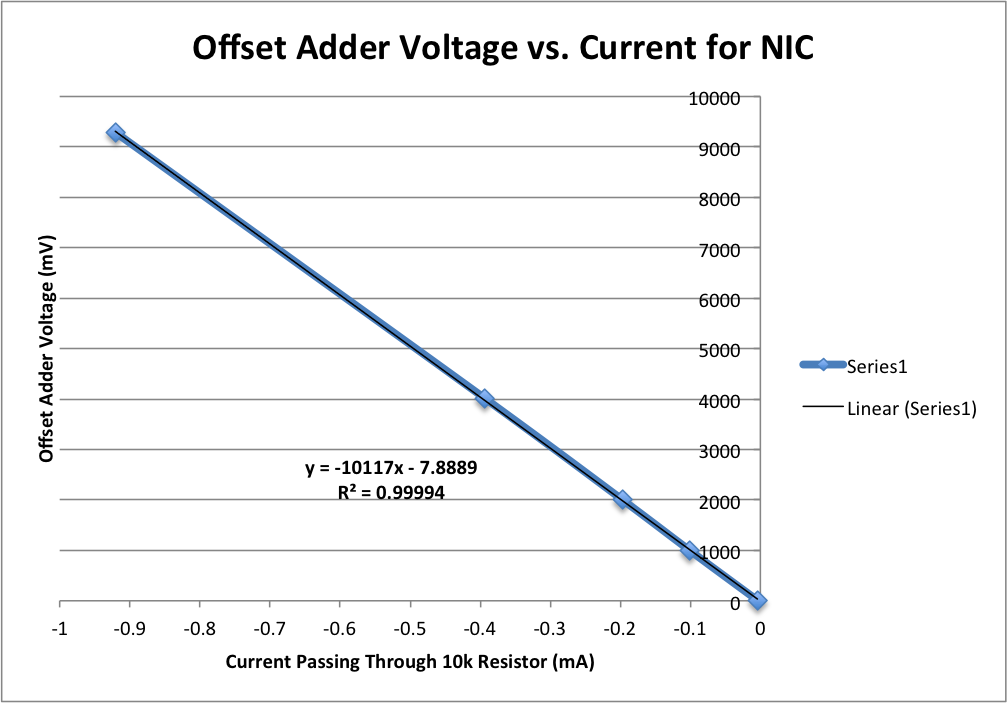
\includegraphics[scale = 0.5]{1b.png}
            \caption{Plot of the offset adder voltage versus the current flowing through the 10k resistor for the NIC}
            \label{fig:my_label}
        \end{figure}
    And we see that if we fit a line to the data, the NIC's impedance is the slope of the line, and this value is -10117 $\Omega$, which means that the NIC appears to behave like a -10k resistor.
    %2
    \subsection{Gyrator}
    \begin{figure}[H]
        \centering
        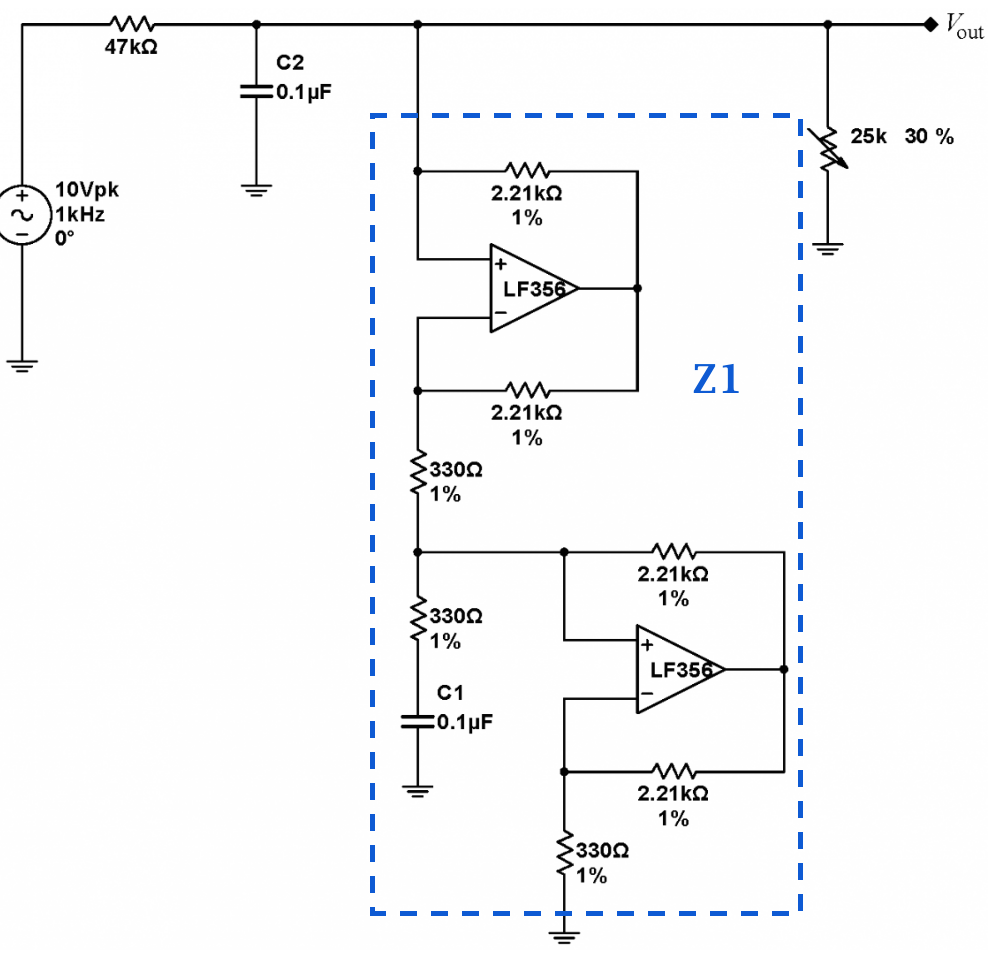
\includegraphics[scale = 0.6]{2.png}
        \caption{Gyrator \cite{lab7} ($Z_1$ is the equivalent input impedance of the enclosed region)}
        \label{fig:my_label}
    \end{figure}
    \begin{table}[H]
        \centering
        \caption{Resistances used in the circuit}
        \label{my-label}
        \begin{tabular}{ll}
        \textbf{$R_{theoretical} (\Omega)$} & \textbf{$R_{meas} (\Omega)$} \\ \hline
        330 & 329.4 \\
        330 & 329.7 \\
        330 & 328.2 \\
        2.2k & 2.1971k \\
        2.2k & 2.1938k \\
        2.2k & 2.2034k \\
        2.2k & 2.1928k
        \end{tabular}
        \end{table}
    Building the circuit in the above figure, the resistors used in this circuit are depicted in the above table. Driving this circuit with various frequency sine waves, and we found the resonance frequency to be 4.6 kHz for a $V_{in}$ of 10 $V_{pp}$ and a $V_{out}$ of 744 mV.\\\indent We can treat this circuit as a fake RLC circuit, with the imaginary inductor of impedance $Z_1 = j\omega R^{2}*C_1$ (see problem [1.14] for derivation)(j is imaginary) having a fake inductance of $L = C_1 * R^{2}$ \cite{lab7}, where $C_1$ is the 0.1 $\mu$F and R is the 330$\Omega$ resistor, as featured in the above figure. For an resonant RLC circuit, the calculated resonant frequency is $f = \frac{1}{2\pi \sqrt{LC_2}} = \frac{1}{2\pi \sqrt{R^{2}*C_1*C_2}} = \frac{1}{2\pi \sqrt{330\Omega*0.1\mu F*0.1\mu F}} \approx 4.82 kHz$. We see that the measured resonant frequency is lower than expected, but in the correct general range.\\\indent Thus, returning to our analysis on measured values, the voltage we used to find our rolloff points were $\frac{744mV}{\sqrt{2}} \approx 526 mV$. The corresponding rolloff frequencies were at 4.39 kHz and 4.81 kHz. We calculated our Q value to be:
    \begin{equation}
        Q = \frac{\omega}{\Delta \omega} = \frac{f_{resonant}^{measured}}{\Delta f} = \frac{4.6kHz}{\frac{4.81 kHz - 4.39 kHz}{2}} \approx 21.9
    \end{equation}
    where $\Delta f$ is a half-width of resonance/output curve.\\\indent We can also calculate the approximate Q by using a definition from lab 2 that Q is $2*\pi * $the "number of times by which the resonator will ring or oscillate after it has been hit with an impulse excitation before the voltage drops to 1/e" \cite{lab2}. We drove the circuit with a 10 Hz, high amplitude square wave, and we noticed that the amplitude (not peak-peak) of the first ring was 62.2 mV, and we counted the number of rings until the voltage dropped below $\frac{62.2 mV}{e}\approx 22.88mV$. This occurred after 4 rings. So applying the formula above, we see that:
    \begin{equation}
        Q \approx 2\pi * 4 \approx 25.13
    \end{equation}
    which is a little different from the other measured Q value.\\\indent Changing the 0.1 $\mu$F capacitor C1 to 1 $\mu$F, and we see that the resonant frequency of the circuit decreases to 1.52 kHz, which is an appropriate change because inputting this change of capacitance into our expected resonant frequency formula, and we find that $f_{expected} = \frac{1}{2\pi \sqrt{R^{2}*C_1*C_2}} = \frac{1}{2\pi \sqrt{330\Omega*1\mu F*0.1\mu F}} \approx 1.53 kHz$, which is very close to the found resonant frequency. Thus, the resonant frequency of the circuit changes appropriately as $C_1$ is switched out.
    \\\indent The 47k resistor of the circuit measured to be 46.5k and the capacitors used in this circuit were 0.1046$\mu$F, 0.1062$\mu$F, and 0.96306$\mu$F.
    
    %3
    \subsection{Relaxation Oscillator}
    \begin{figure}[H]
        \centering
        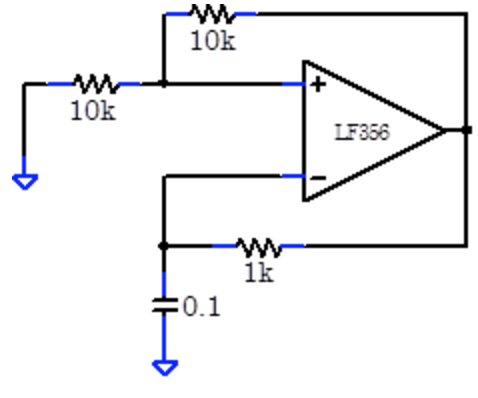
\includegraphics[scale = 0.6]{3.png}
        \caption{Relaxation Oscillator \cite{lab7}}
        \label{fig:my_label}
    \end{figure}
    Building the relaxation oscillator above, we attain a scope traces of the image of the op amp and capacitor outputs:
    \begin{figure}[H]
        \centering
        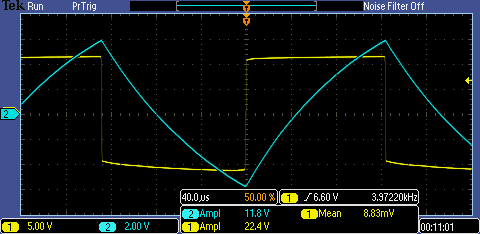
\includegraphics[scale = 0.7]{3a.PNG}
        \caption{Scope Trace of Op Amp Output Signal ($V_{out}$ is red) and the voltage across the capacitor ($V_-$, color is yellow)}
        \label{fig:my_label}
    \end{figure}
    We see that the op amp output signal is channel 1 of the scope trace and the capacitor signal is channel 2.\\\indent
    Diving into the theory behind this circuit, we can treat the connections from $V_{out}$ to ground on either side as voltage dividers. As such, we find that $V_+ = \frac{V_{out}}{2}$. Essentially what is happening is that the capacitor in the circuit is either being charged or discharged by the voltage leaving from $V_{out}$. $V_{out}$ can either have a HIGH or LOW setting, as this value is determined by a comparator input, that is, $V_{out}$ is HIGH if $V_- < V_+$ and $V_{out}$ is LOW if $V_- > V_+$. A HIGH output value will begin to charge the capacitor, and a LOW output value will discharge the capacitor. We see that in this case, the HIGH value is out 12V power supply value and our LOW value is our -12V power supply. We see that when the output is HIGH, $V_+ = 6V$ and the capacitor is charging ($V_C = V_-$), that is, $V_-$ is increasing towards $V_+$. When $V_-$ increases past $V_+$, the output switches to LOW, $V_+ = -6V$, and the capacitor discharges. We will analyze the discharging sequence of the capacitor to find the resonant frequency of the circuit. We know that the discharging voltage across the capacitor is:
    \begin{equation}
        V_- = V_{initial} + (V_{out}-V_{initial})(1-e^{-\frac{t}{\tau}})
    \end{equation}
    with $\tau = 1k\Omega*0.1\mu F$. This equation simplifies to:
    \begin{equation}
        V_- = 18e^{-\frac{t}{\tau}}-12 volts
    \end{equation}
    after we set $V_{out} = -12V$ and $V_{initial} = 6V$ ($V_-$ is initially 6V when capacitor begins to discharge). We want to see when this voltage drops below $V_+ = -6V$. So setting the above equation for $V_-$ equal to -6V, we solve for t and find that t = $\tau ln(3)$. Since the capacitor takes as long to charge as it does to discharge, the period of oscillation is T = 2t = $2\tau ln(3)$, and thus the calculated resonant frequency of the circuit is f = $\frac{1}{2*\tau*ln(3)}$ = $\frac{1}{2*1k\Omega*0.1\mu F*ln(3)} \approx 4.55 kHz$. Looking at figure 6, we see that the period of oscillation is 250$\mu$s, corresponding to a frequency of $\approx$ 4kHz, which is within a reasonable range of our predicted value (off by relative error of 11$\%$).
    
    %4
    \subsection{Filters}
        \subsubsection{Written Portion}
        \begin{figure}[H]
            \centering
            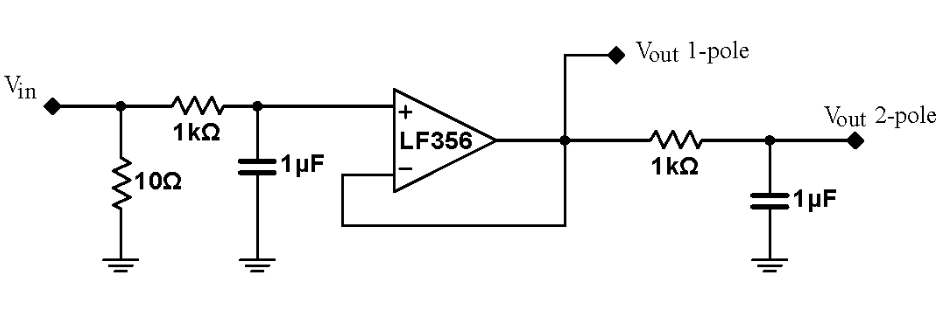
\includegraphics[scale = 0.6]{41.png}
            \caption{Multistage Filter \cite{lab7}}
            \label{fig:my_label}
        \end{figure}
        My partner and I built the above circuit and casually explored the behavior of the circuit near a driving frequency of 160 Hz, and found that for frequency values larger than this, $V_{out} 2-pole$'s signal became more strongly attenuated than the 1-pole output.
        \begin{figure}[H]
            \centering
            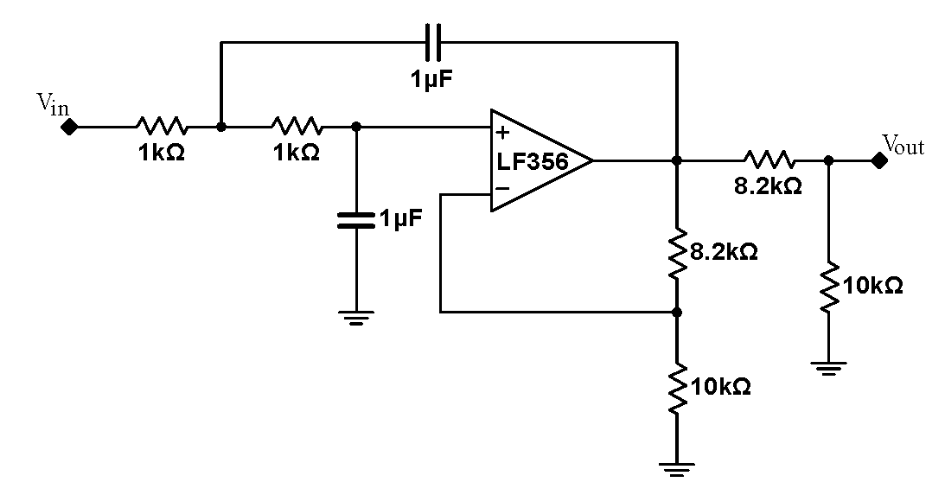
\includegraphics[scale = 0.6]{42.png}
            \caption{Chebyshev Sallen-Key filter \cite{lab7}}
            \label{fig:my_label}
        \end{figure}
        Having constructed the Chebyshev Sallen-Key filter above, we explored the output of this circuit near the 160 Hz driven frequency, and found that the circuit behaved as a low pass filter and began to very sharply attenuate the signal after this cutoff point.
        \subsubsection{Signatured Part of This Section}
        See Signature Page
    %5
    \subsection{Absolute Value}
        See signature page
    %6
    \subsection{Logarithm}
    \begin{figure}[H]
        \centering
        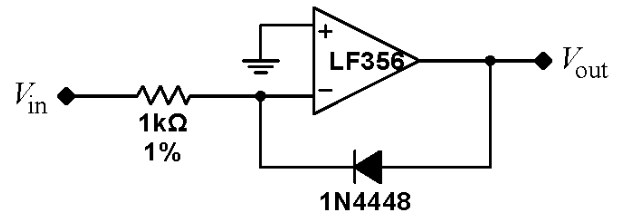
\includegraphics[scale = 0.6]{6.png}
        \caption{Logarithm Circuit \cite{lab7}}
        \label{fig:my_label}
    \end{figure}
    We built the logarithm circuit as depicted above and recorded various $V_{in}$ and $V_{out}$ values and plotted the data for -$V_{in}$ vs $V_{out}$. Below is the measured data:
        \begin{table}[H]
            \centering
            \caption{$V_{in}$ and $V_{out}$ measured values for Logarithm circuit}
            \label{my-label}
            \begin{tabular}{lll}
            \textbf{-Vin (V)} & \textbf{Vin (V)} & \textbf{Vout (V)} \\ \hline
            0.0349 & -0.0349 & 0.3366 \\
            0.225 & -0.225 & 0.545 \\
            0.792 & -0.792 & 0.6097 \\
            0.864 & -0.864 & 0.619 \\
            1.439 & -1.439 & 0.6403 \\
            1.92 & -1.92 & 0.652 \\
            3.37 & -3.37 & 0.682 \\
            8.15 & -8.15 & 0.7263 \\
            9.567 & -9.567 & 0.7364
            \end{tabular}
            \end{table}
    And -$V_{in}$ plotted against $V_{out}$:
    \begin{figure}[H]
        \centering
        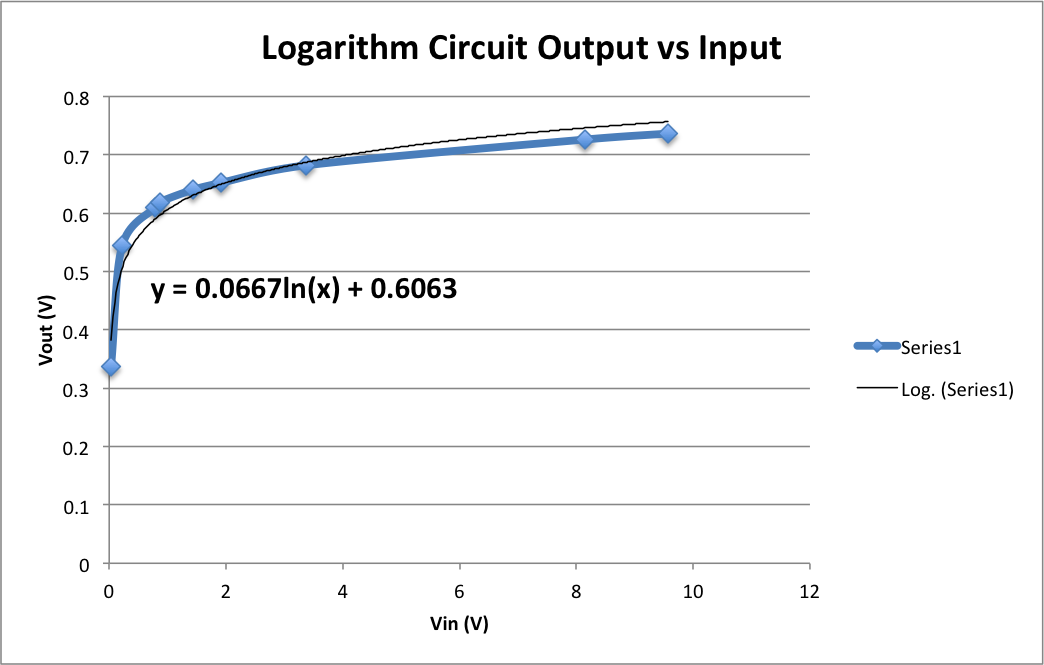
\includegraphics[scale = 0.7]{6a.png}
        \caption{Graph of -$V_{in}$ and $V_{out}$ measured values for Logarithm circuit}
        \label{fig:my_label}
    \end{figure}
    Finding the curve of best fit to the data, and we see that the data is closely modelled by:
    \begin{equation}
        V_{out} = 0.0667 * ln(-V_{in}) + 0.6063
    \end{equation}
    We would normally expect to find the curve derived in the prelab:
    \begin{equation}
        V_{out} = \frac{nKT}{e} * ln(\frac{-V_{in}}{i_{sat} R})
    \end{equation}
    Thus, we see that vertical and horizontal scaling factors have transformed this data, so the data has been transformed from a basic logarithm function, and that our expected curve has been shifted upwards by $\sim$ 0.6V. So we will need to scale and offset the data to make it match a true logarithm. We found a statistical correlational $R^{2}$ value of 0.95, which has high predictive strength.
    
    %7
    \subsection{Multiplier and Shifter}
    \begin{figure}[H]
        \centering
        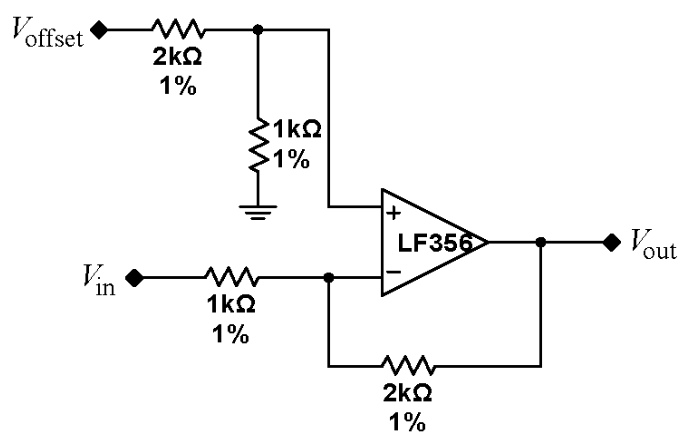
\includegraphics[scale = 0.6]{71.png}
        \caption{Multiplier and Shifter Circuit \cite{lab7}}
        \label{fig:my_label}
    \end{figure}
    \begin{figure}[H]
        \centering
        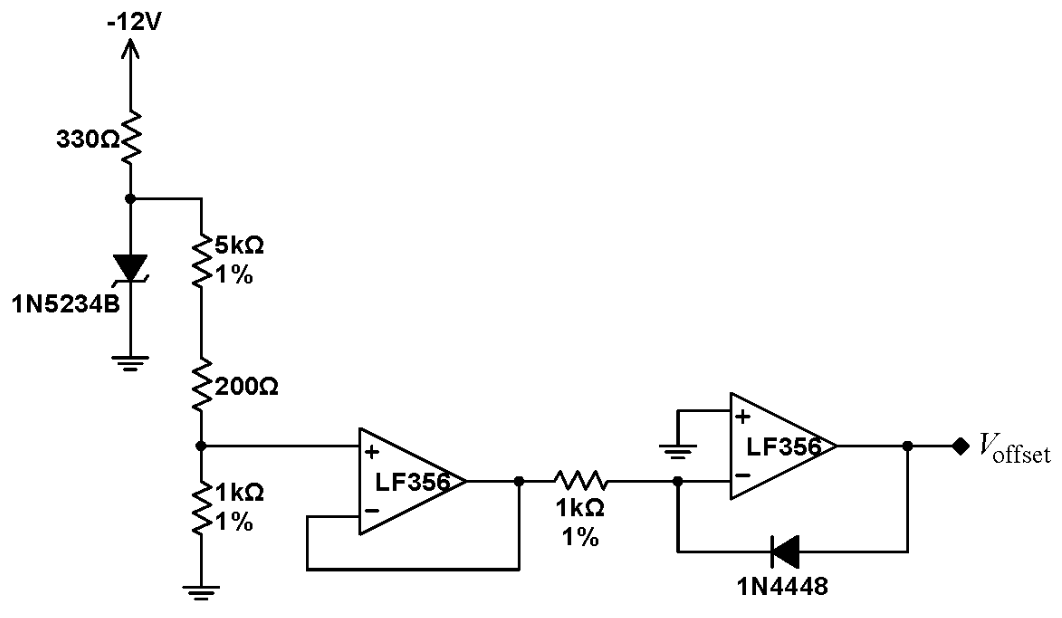
\includegraphics[scale = 0.6]{72.png}
        \caption{Circuit producing $V_{off}$ \cite{lab7}}
        \label{fig:my_label}
    \end{figure}
        We built the two circuits above and linked $V_{offset}$ (figure 12) to the main multiplier/shifter circuit (figure 11). With out setup, we measured the output of the first op amp to be -1.02V, and the output of figure 12 ($V_{offset}$) to be 612 mV, which were both the values that we were expecting. We then drove the logarithm circuit with approximately 600 mV, and measured the output of the multiplier/shifter to be -1.12V, which demonstrates that the output was doubled, inverted, and vertically offset by the proper amount.
    %8
    \subsection{Exponentiator}
    \begin{figure}[H]
        \centering
        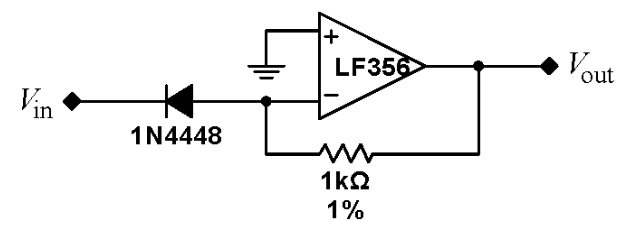
\includegraphics[scale = 0.6]{8.png}
        \caption{Exponentiator Circuit \cite{lab7}}
        \label{fig:my_label}
    \end{figure}
    We built the exponentiator circuit demonstrated above, and collected the following data points for the input and output of the circuit:
    \begin{table}[H]
        \centering
        \caption{$V_{in}$ and $V_{out}$ measured values for Exponentiator circuit}
        \label{my-label}
        \begin{tabular}{lll}
        \textbf{-Vin (mV)} & \textbf{Vin (mV)} & \textbf{Vout (mV)} \\ \hline
        5 & -5 & 10 \\
        298 & -298 & 12 \\
        495 & -495 & 172 \\
        658 & -658 & 2910 \\
        697 & -697 & 6000 \\
        703 & -703 & 7800 \\
        714 & -714 & 9590
        \end{tabular}
        \end{table}
    We plotted the data and fit an exponential curve to the data with a correlational $R^{2}$ value of 0.887:
    \begin{figure}[H]
        \centering
        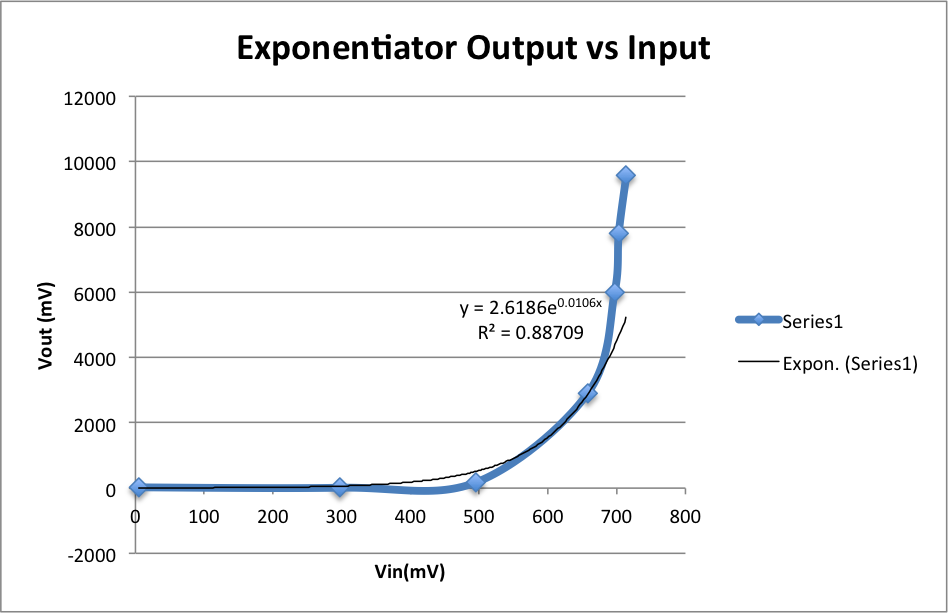
\includegraphics[scale = 0.7]{8a.png}
        \caption{Plot of $V_{in}$ vs $V_{out}$ measured values for Exponentiator circuit}
        \label{fig:my_label}
    \end{figure}
    we see that the data begins to diverge at really large input voltages. The data appears to look like an exponential, so we see that the circuit is behaving as expected.
    
    %9
    \subsection{Squarer}
        See signature page
    %10
    \subsection{Time Averager}
    \begin{figure}[H]
        \centering
        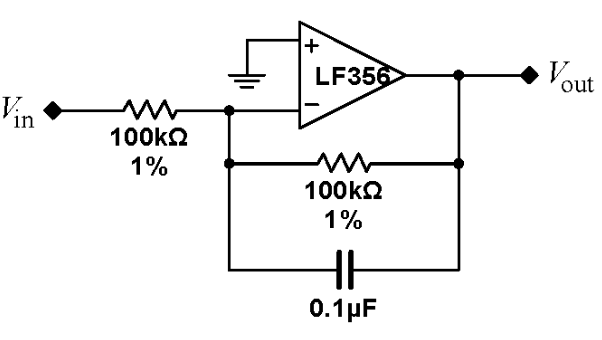
\includegraphics[scale = 0.6]{10.png}
        \caption{Time Averager Circuit \cite{lab7}}
        \label{fig:my_label}
    \end{figure}
    The time averager, constructed above, was driven with a variety of waveforms, and we noticed that the output of the circuit was the inverse average of the input. For instance, we offset a 5$V_{pp}$ 200kHz sine wave offset by -4V, as depicted in the figure/scope trace below:
    \begin{figure}[H]
        \centering
        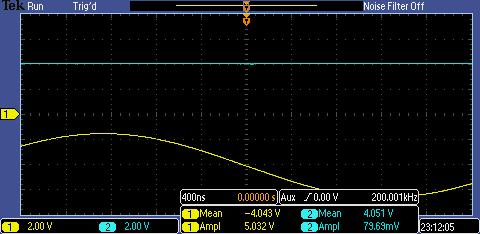
\includegraphics[scale = 0.6]{10b.PNG}
        \caption{Time averager scope trace; $V_{in}$ is yellow, $V_{out}$ is blue}
        \label{fig:my_label}
    \end{figure}
    where channel 1 is the input and channel 2 is the output of the time averager. The mean of the channel 1 output is -4.043V. We expected the circuit to output a DC voltage offset of 4.043, which is the inverse average of the input. We attained a channel 2 output of 4.041 VDC, which is very close to our expected value. Thus, we conclude that the time averager works as it is supposed to function.\\\indent 
    However, we found that the circuit does not work well in the range of low frequencies (as we investigated by trying many different wave forms), for at these frequencies, instead of just getting a DC signal output, we attained an attenuated but noticeable AC signal about the DC offset we were looking for. We established an artificial cutoff for the frequency by which all the outputs of all frequencies above would produce proper DC-looking output time-averaged signals. We took a sine wave and varied its frequency and looked at the output signal until we noticed that the peak-peak amplitude of the output wave was less than 20 mV (our artificial cutoff) about the fixed time averaged DC value, which we then called this signal the approximate DC signal: 
    \begin{figure}[H]
        \centering
        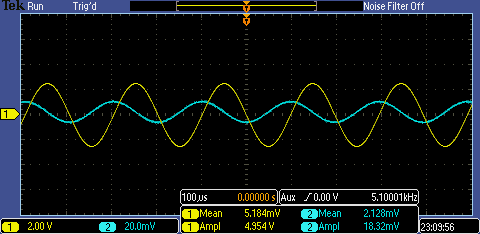
\includegraphics[scale = 0.7]{10a.PNG}
        \caption{Time averager circuit attenuating the amplitude of the output wave for high frequencies (5.1 kHz)}
        \label{fig:my_label}
    \end{figure}
    This occurred at a frequency of 5.1 kHz for a 5 $V_{pp}$ input sine wave, as we notice in the figure above, whose 4.954 $V_{pp}$ input sine wave was attenuated to $18.32mV$ output, and with an offset input sine wave, the DC inverted time averaged output can be found as in figure 16.\\\indent 
    The capacitor and the 100k in parallel help set this frequency range because looking at the equation from the lab sheet \cite{lab7}:
    \begin{equation}
        \displaystyle\left<H\right>(t)=\frac{1}{\tau}\int_{-\infty}^{t}H(t^\prime)\exp\left(\frac{t^\prime-t}{\tau}\right)\,dt^\prime
    \end{equation}
    $\tau = RC$ is the time constant of the time averaging signal, by which R is the 100k resistor and C is the 0.1 $\mu$F capacitor (see [1.17] for derivation). We see that at high frequencies, $t^\prime - t \approx 0$, and the exponential term in the integrand essentially disappears (i.e. turns into 1), turning the circuit into a proper time averager:
    \begin{equation}
        \displaystyle\left<H\right>(t)=\frac{1}{\tau}\int_{-\infty}^{t}H(t^\prime)\,dt^\prime
    \end{equation}
    However, at low frequencies, the impedance of the capacitor, $\frac{j}{\omega C}$, blows up towards infinity, ensuring that almost all of the current flows through the feedback resistor. In this case, $t^\prime - t$ is on the same order of magnitude as $\tau$, and the circuit behaves more like an inverted follower. We see that this disturbance (increased following/ larger amplitude sine wave output) is really pronounced when $t^\prime - t = \tau = RC = 100k\Omega *0.1\mu F \approx 10ms$, corresponding to driven frequencies of $\frac{1}{10ms} \approx 100Hz$. When the circuit is driven at frequencies on a similar order of magnitude, the circuit experiences "failure", which is why we established our unofficial cutoff frequency to be at about 5.1 kHz, where the order of magnitude of the driven frequency is high enough such that the circuit does not experience significant inverted follower effects. At any frequency above our unofficial cutoff, we can call the output "DC".
    
    %11
    \subsection{Square Rooter}
    \begin{figure}[H]
        \centering
        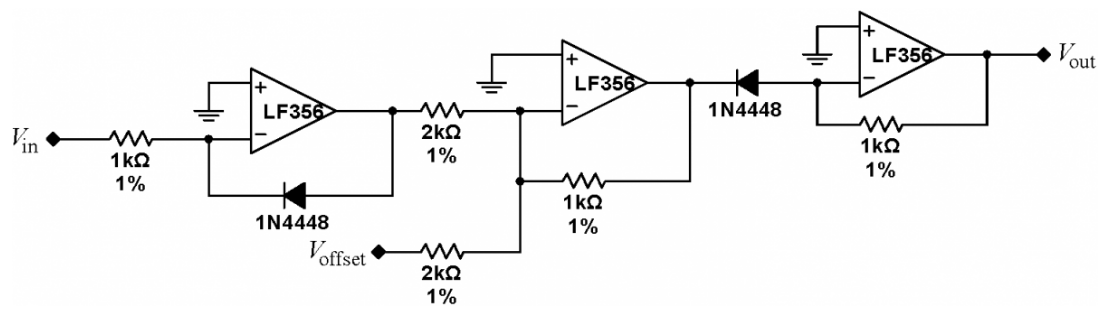
\includegraphics[scale = 0.6]{11.png}
        \caption{Square Rooter Circuit \cite{lab7}}
        \label{fig:my_label}
    \end{figure}
    The square rooter depicted in the above figure was built, and each section was debugged separately and produced the proper outputs. We drove the circuit with a series of negative DC input voltages and attained the following output data points:
        \begin{table}[H]
            \centering
            \caption{Square Rooter Input and Output (measured vs expected) Voltages}
            \label{my-label}
            \begin{tabular}{lll}
            \textbf{$V_{in}$ (V)} & \textbf{$V_{out}measured$(V)} & \textbf{$V_{out}expected$(V)} \\ \hline
            -2.27 & 1.415 & 1.506651917 \\
            -1.751 & 1.254 & 1.323253566 \\
            -1.21 & 1.123 & 1.1 \\
            -1.035 & 1.062 & 1.017349497 \\
            -0.7081 & 0.8135 & 0.841486779 \\
            -0.491 & 0.6822 & 0.700713922 \\
            -0.19 & 0.442 & 0.435889894 \\
            -0.1297 & 0.3619 & 0.360138862
            \end{tabular}
            \end{table}
    In the above figure, we have the measured $V_{in}$, the measured $V_{out}$ and the predicted $V_{out}$ if $V_{out} = \sqrt{-V_{in}}$ for the corresponding $V_{in}$ values. The data is plotted below:
    \begin{figure}[H]
        \centering
        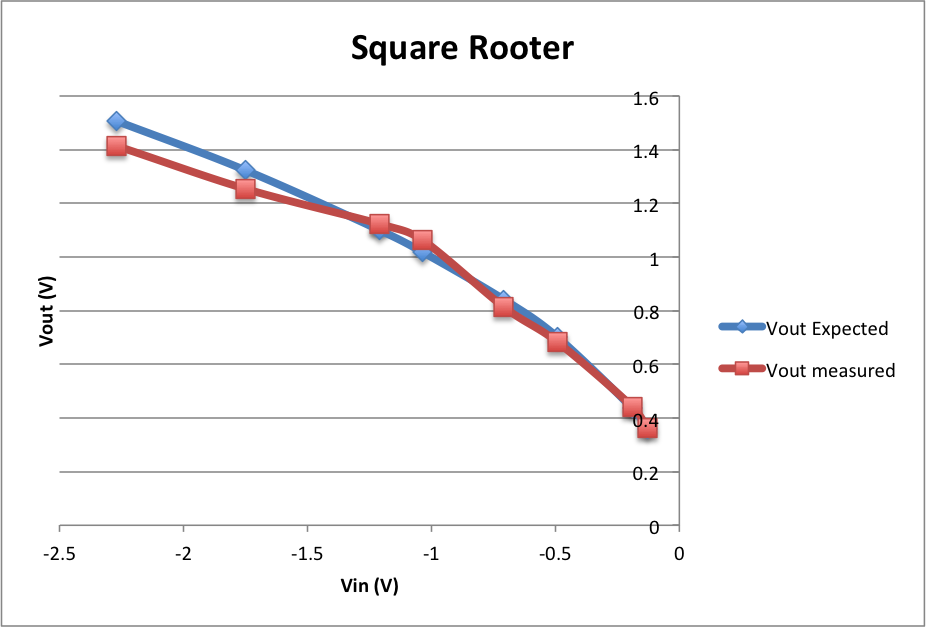
\includegraphics[scale = 0.6]{11a.png}
        \caption{Plotted $V_{in}$ vs. $V_{out}$ for square rooter}
        \label{fig:my_label}
    \end{figure}
    Thus, we see that the module does a pretty good job of taking the square root of the input signal, as the expected curve closely aligns with our measured value with error values deviating on both sides of the expected curve. Table 5 shows that the measured and expected values are quite close to one another.
    %12
    \subsection{RMS Converter: No Averaging}
        See signature page
    %13
    \subsection{RMS Converter}
        See signature page
    %14
    \subsection{Gyrator Analysis}
    \begin{figure}[H]
        \centering
        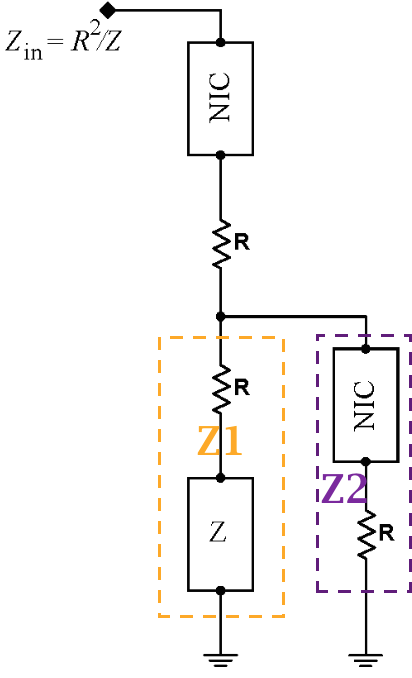
\includegraphics[scale = 0.6]{14a.png}
        \caption{Simplified gyrator \cite{lab7}, analyzing components to find input impedance}
        \label{fig:my_label}
    \end{figure}
    We want to prove that the input impedance of the gyrator, simplified to the above circuit diagram, is $Z_{in} = \frac{R^{2}}{Z}$. We begin our analysis by identifying impedances $Z_1$ and $Z_2$, each indicated in the color coded regions above:
    \begin{equation}
        Z_1 = R + Z
    \end{equation}
    \begin{equation}
        Z_2 = -R
    \end{equation}
    $Z_2$ is such because the negative impedance converter changed the R component below it into -R impedance. We add up the two impedances in parallel to find:
    \begin{equation}
        Z_3 = \frac{Z_1 * Z_2}{Z_1 + Z_2} = \frac{(R+Z)*(-R)}{R+Z-R} = \frac{-R^{2}}{Z} - R
    \end{equation}
    Now, the equivalent impedance below the first NIC in the circuit is:
    \begin{equation}
        Z_{eq} = R + Z_3 = R + \frac{-R^{2}}{Z} - R = \frac{-R^{2}}{Z}
    \end{equation}
    where the R added is the resistance immediately below the first NIC. The first NIC causes the sign of the equivalent impedance below to switch from positive to negative, and thus:
    \begin{equation}
        Z_{in} = -Z_{eq} = \frac{R^{2}}{Z}
    \end{equation}
    which is the intended result. We see that the circuit setup of the gyrator (figure 4) utilizes this setup, and thus, the circuit behaves as expected.
    %15
    \subsection{Absolute Value Analysis}
    \begin{figure}[H]
        \centering
        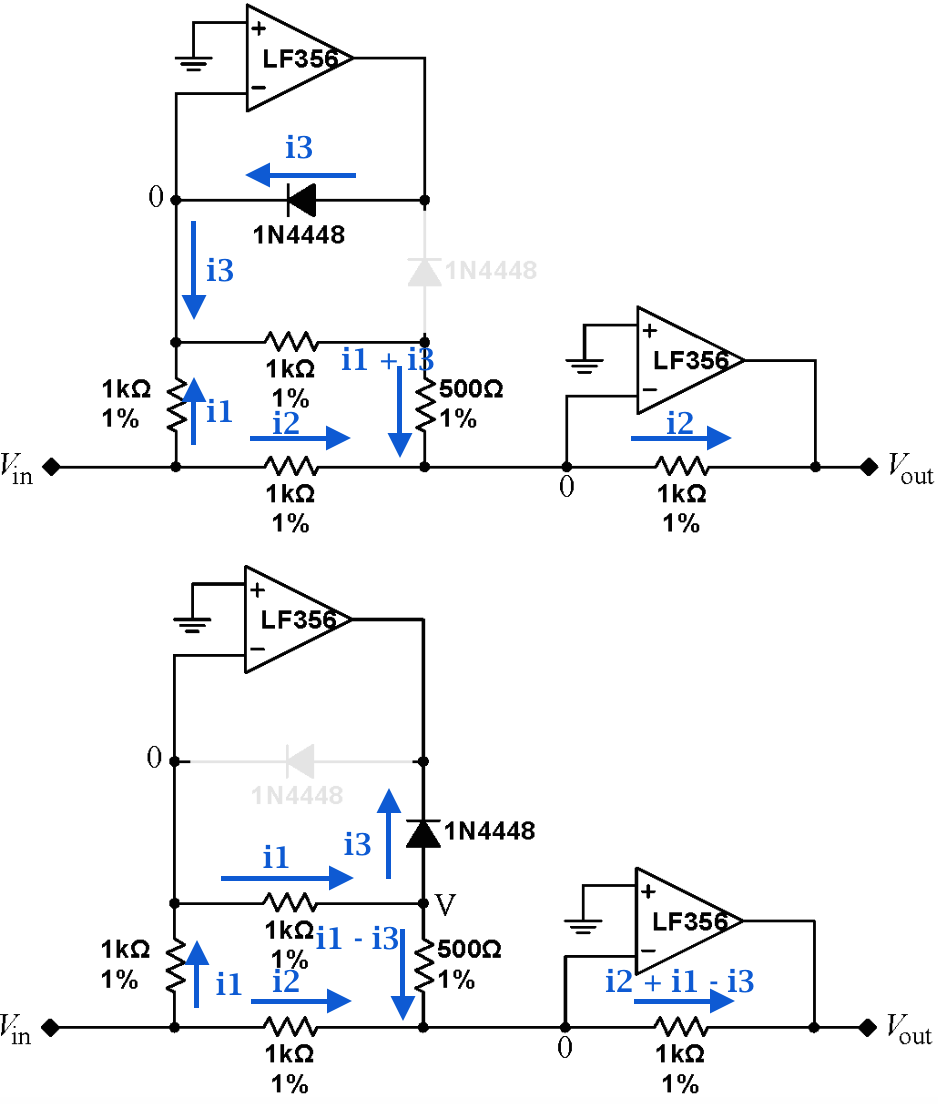
\includegraphics[scale = 0.6]{15.png}
        \caption{Absolute Value Circuit \cite{lab7} with currents labelled; diagrams 1 and 2 (each with a diode removed; currents labelled)}
        \label{fig:my_label}
    \end{figure}
    \begin{figure}[H]
        \centering
        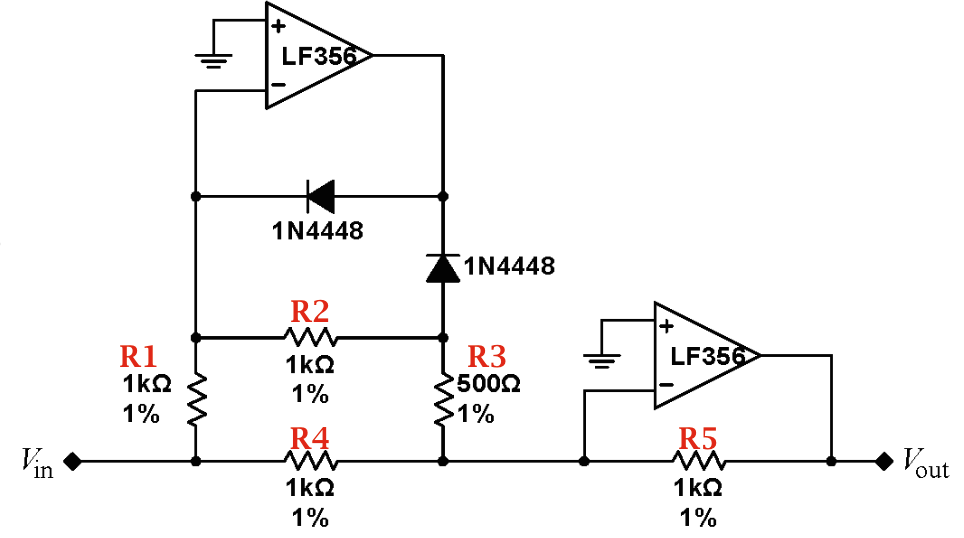
\includegraphics[scale = 0.6]{15a.png}
        \caption{Absolute Value Circuit \cite{lab7} with Resistors Labelled}
        \label{fig:my_label}
    \end{figure}
    We analyze the absolute value circuit using the above two figures. We have denoted currents in figure 21 (different numbering schemes for different diagrams) and resistance values in figure 22 (the resistor numbering describes the resistors for the diagrams in figure 21) for extra clarification for the analysis. \\\indent For our first analysis, we set $V_{in} < 0$, and thus consider the top diagram of figure 21 with the resistor names of figure 22. We see that $i_1 + i_3$ is the current across $R_3$, the 500$\Omega$ resistor. We note that 
    \begin{equation}
        i_1 = \frac{V_{in}}{R_1}
    \end{equation}
    and 
    \begin{equation}
        i_2 = \frac{V_{in}}{R_4}
    \end{equation}
    we denote the direct voltage output of the first op amp as $V_o$, and it has already been assumed that this quantity is greater than 0V. We also notice that $V_-$ of the first and second op amps are 0V (op amp golden rules), and thus, the voltage drop across $R_2$ and $R_4$ is 0V, so the current passing through $R_2$ and $R_4$ ($R_3$ being the 500$\Omega$ resistor), $i_1 + i_3$, is 0A. There is also no current entering $V_-$ of the second op amp, as per the op amp golden rules of op amps. Now, we have enough information to attempt to find $V_{out}$ given that $V_{in} < 0V$. Following the path of $i_2$, we see that:
    \begin{equation}
        i_2 = \frac{V_{in} - V_{out}}{R_4 + R_5}
    \end{equation}
    and rearranging and substituting for $i_2$, and we find that:
    \begin{equation}
        V_{out} = V_{in} - i_2 (R_4 + R_5) = V_{in} - \frac{V_{in}*(R_4 + R_5)}{R_4}
    \end{equation}
    and plugging in $R_4 = R_5 = 1k$:
    \begin{equation}
        V_{out} = -V_{in}
    \end{equation}
    which is the result we were looking for for an absolute value circuit.
    \\\indent Now, analyzing the case when $V_{in} > 0$, we turn to the circuit of the second diagram of figure 21, with new current labels. First, we can deduce by inspection that:
    \begin{equation}
        \begin{array}{lllll}
            i_1 & = & \frac{V_{in}}{R_1} & = & \frac{-V}{R_2}\\
            i_2 & = & \frac{V_{in}}{R_4} &  &  \\
            i_1 - i_3 & = & \frac{V}{R_3} &  &  
        \end{array}
    \end{equation}
    given that $V_{in} > 0V$ and $V_{o} < 0V$. The voltage V must be:
    \begin{equation}
        V = \frac{-R_2 * V_{in}}{R_1} = -V_{in}
    \end{equation}
    The total current entering the $V_-$ of the second op amp is still 0V per golden rules of op amps, but the voltage passing through $R_4$ is $i_2$ and through $R_5$ is $i_2 + i_1 - i_3$, and we see by analyzing the voltage drop between $V_-$ of the second op amp and $V_{out}$ that:
    \begin{equation}
        V_{out} = -R_5 * (i_2 + i_1 - i_3) 
    \end{equation}
    and substituting for the three currents that:
    \begin{equation}
        V_{out} = -R_5 * (\frac{V_{in}}{R_4} + \frac{V}{R_3}) = -R_5 * (\frac{V_{in}}{R_4} + \frac{-V_{in}}{R_3}) = -R_5 * V_{in} (\frac{1}{R_4} - \frac{1}{R_3})
    \end{equation}
    And plugging in $R_4 = R_5 = 1k$ and $R_3 = 500\Omega$ that:
    \begin{equation}
        V_{out} = -1k * V_{in} (\frac{1}{1k} - \frac{1}{0.5k}) = V_{in}
    \end{equation}
    So we see that in the case that $V_{in} > 0V$, that $V_{out} = V_{in} > 0V$.
    \\\indent In summary, for $V_{in} <$ 0V, we see that $V_{out} = -V_{in}$; and for $V_{in} >$ 0V, we see that $V_{out} = V_{in}$, which directly demonstrates that the circuit performs as desired. That is, given the preceding analysis:
    \begin{equation}
        V_{out} = |V_{in}|
    \end{equation}
    
    %16
    \subsection{Squarer Analysis}
    \begin{figure}[H]
        \centering
        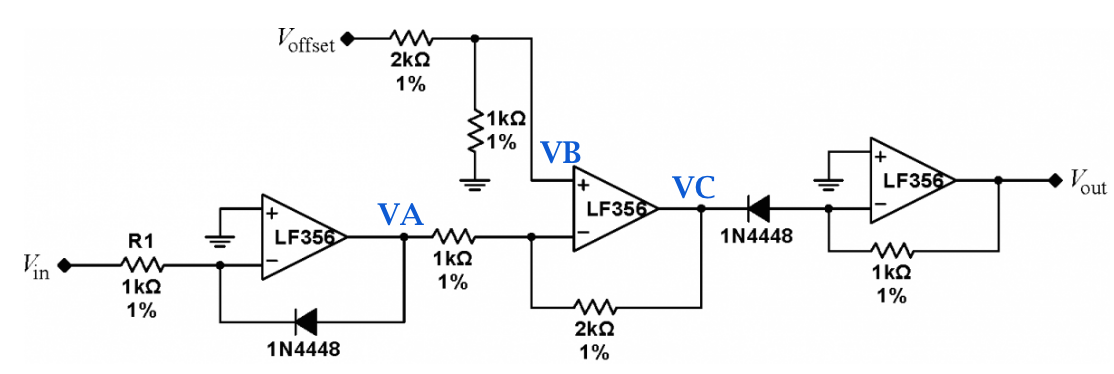
\includegraphics[scale = 0.6]{16.png}
        \caption{Squarer Circuit \cite{lab7} with voltages $V_A$, $V_B$, and $V_C$ labelled}
        \label{fig:my_label}
    \end{figure}
    We will analyze the above squarer with voltage points $V_A$, $V_B$ and $V_C$ marked on the above figure. We know the current (i, left to right) passing through the diode is \cite{lab7}:
    \begin{equation}
        i(V_{A}) = - i_{sat}e^{\frac{eV_{A}}{nKT}} = \frac{V_{in}}{1k}
    \end{equation}
    which defines the input and output of the logarithm part of the squarer.\\\indent
    And looking at the last part of the circuit, the exponentiator, we look at the circuit components between $V_C$ and $V_{out}$ and notice that the current passing through this diode is \cite{lab7}:
    \begin{equation}
        i(V_{C}) = i_{sat}e^{\frac{e(-V_{C})}{nKT}} = \frac{V_{out}}{1k}
    \end{equation}
    which defines the inputs and outputs of the exponentiator part of the squarer. \\\indent Now we take a look at the middle component between $V_A$ and $V_C$, the multiplier and shifter. We see that $V_B = \frac{1k * V_{off}}{2k + 1k} = \frac{V_{off}}{3}$. We also see that by the golden rules of op amps, $V_- = V_+ = V_B$. Then we also see by analyzing the voltage drops across the feedback resistor and the resistor feeding into $V_-$ of the second op amp, and we see that:
    \begin{equation}
        \frac{V_A - V_B}{1k} = \frac{V_B - V_C}{2k}
    \end{equation}
    with some rearrangement:
    \begin{equation}
        V_C = 3V_B - 2V_A
    \end{equation}
    We can see from eq.(25) that:
    \begin{equation}
        V_A = \frac{nKT}{e} ln(\frac{-V_{in}}{i_{sat}*1k})
    \end{equation}
    So plugging in for $V_B$ and $V_A$:
    \begin{equation}
        V_C = V_{off} - 2*\frac{nKT}{e} ln(\frac{-V_{in}}{i_{sat}*1k})
    \end{equation}
    And plugging in $V_C$ into the equation for $V_{out}$, we get:
    \begin{equation}
        V_{out} = i_{sat}*1k*\mathit{e}^{-\frac{eV_{C}}{nKT}} = i_{sat}*1k*\mathit{e}^{\frac{e(-V_{off} + 2*\frac{nKT}{e} ln(\frac{-V_{in}}{i_{sat}*1k}))}{nKT}} = i_{sat}*1k*\mathit{e}^{\frac{-e*V_{off}}{nKT}}*\mathit{e}^{ln(\frac{V_{in}^{2}}{(i_{sat}*1k)^{2}})}
    \end{equation}
    And thus:
    \begin{equation}
        V_{out} = \frac{V_{in}^{2}}{i_{sat}*1k}*\mathit{e}^{\frac{-e*V_{off}}{nKT}}
    \end{equation}
    Now setting n=2, kT $\approx \frac{1}{40}eV$, $V_{off} \approx 0.6V$, and from lab 3 \cite{lab3}, using $i_{sat} = 2.7*10^{-5} mA$ (which varies based on particular diodes), and plugging in these results into $V_{out}$, we can quickly deduce that $i_{sat}*1k \sim \frac{-e*V_{off}}{nKT}$, and we find that:
    \begin{equation}
        V_{out} \approx V_{in}^{2}
    \end{equation}
    for values $V_{in} < 0V$, limited by the domain of the logarithm part of the signal. (NOTE: The 1k mentioned in this section and in other parts of the lab references a 1k$\Omega$ resistor)
    
    
    %17
    \subsection{Averager Analysis}
    \begin{figure}[H]
        \centering
        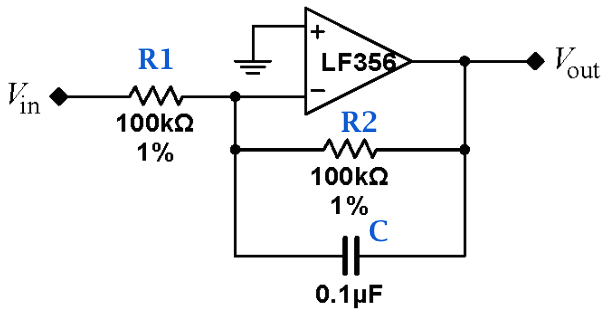
\includegraphics[scale = 0.6]{17.png}
        \caption{Averager Circuit \cite{lab7}, revisited, with resistors and capacitors labelled}
        \label{fig:my_label}
    \end{figure}
    We analyze the time averager above by utilizing the time averager formula for an arbitrary wave signal \cite{lab7}:
    \begin{equation}
        \displaystyle\left<H\right>(t)=-\frac{1}{\tau}\int_{-\infty}^{t}H(t^\prime)\exp\left(\frac{t^\prime-t}{\tau}\right)\,dt^\prime
    \end{equation}
     Where the minus sign was added because of the inverting nature of the circuit. We will denote $<H>$(t) as $V_{out}$ and H(t) as $V_{in}$. A current, $\mathit{i}$, passes from $V_{in}$ rightwards until it is split into $i_1$ and $i_2$ by the feedback impedance components. $i_1$ passes through the capacitor C and travels towards $V_{out}$ and $i_2$ passes rightwards through $R_2$. We can notice that:
    \begin{equation}
        \begin{array}{lll}
            i & = & \frac{V_{in}}{R_1}  \\
            i_1 & = & i - i_2 = i_1*(-C) * \frac{dV_{out}}{dt} = \frac{V_{in}}{R_1} + \frac{V_{out}}{R_2} \\
            i_2 & = & \frac{-V_{out}}{R_2}
        \end{array}
    \end{equation}
    where $V_{out}$ is the opposite of the voltage across the capacitor. This generates the differential equation:
    \begin{equation}
        \frac{dV_{out}}{dt} = \frac{-i_1}{C} = \frac{-V_{in}}{R_1 C} - \frac{V_{out}}{R_2 C}
    \end{equation}
    Now we plug in the particular solution (eq.(34)) for any arbitrary wave function:
    \begin{equation}
        \frac{dV_{out}}{dt} = \frac{d}{dt} (-\frac{1}{\tau}\int_{-\infty}^{t}V_{in}(t^\prime)\exp\left(\frac{t^\prime-t}{\tau}\right)\,dt^\prime) = -\frac{1}{\tau}*(-\mathit{e}^{\frac{-t}{\tau}}*\frac{\int_{-\infty}^{t}V_{in}(t^\prime)\exp\left(\frac{t^\prime}{\tau}\right)\,dt^\prime}{\tau} + \mathit{e}^{\frac{-t}{\tau}}*V_{in}*\mathit{e}^{\frac{t}{\tau}})
    \end{equation}
    Which simplifies to:
    \begin{equation}
        \frac{dV_{out}}{dt} = -\frac{1}{\tau}*(V_{out} + V_{in})
    \end{equation}
    Comparing this to eq.(32), we find that:
    \begin{equation}
        \tau = R_1 C = R_2 C = 100k\Omega * 0.1 \mu F \approx 10 ms
    \end{equation}
    And now we know that the circuit implements eq.(34) and that the circuit time averages for any arbitrary signal. From our prior analysis, eq.(34) is the output of the circuit for any arbitrary input signal.
    
    
\section{Signature Page}
\begin{figure}[H]
    \centering
    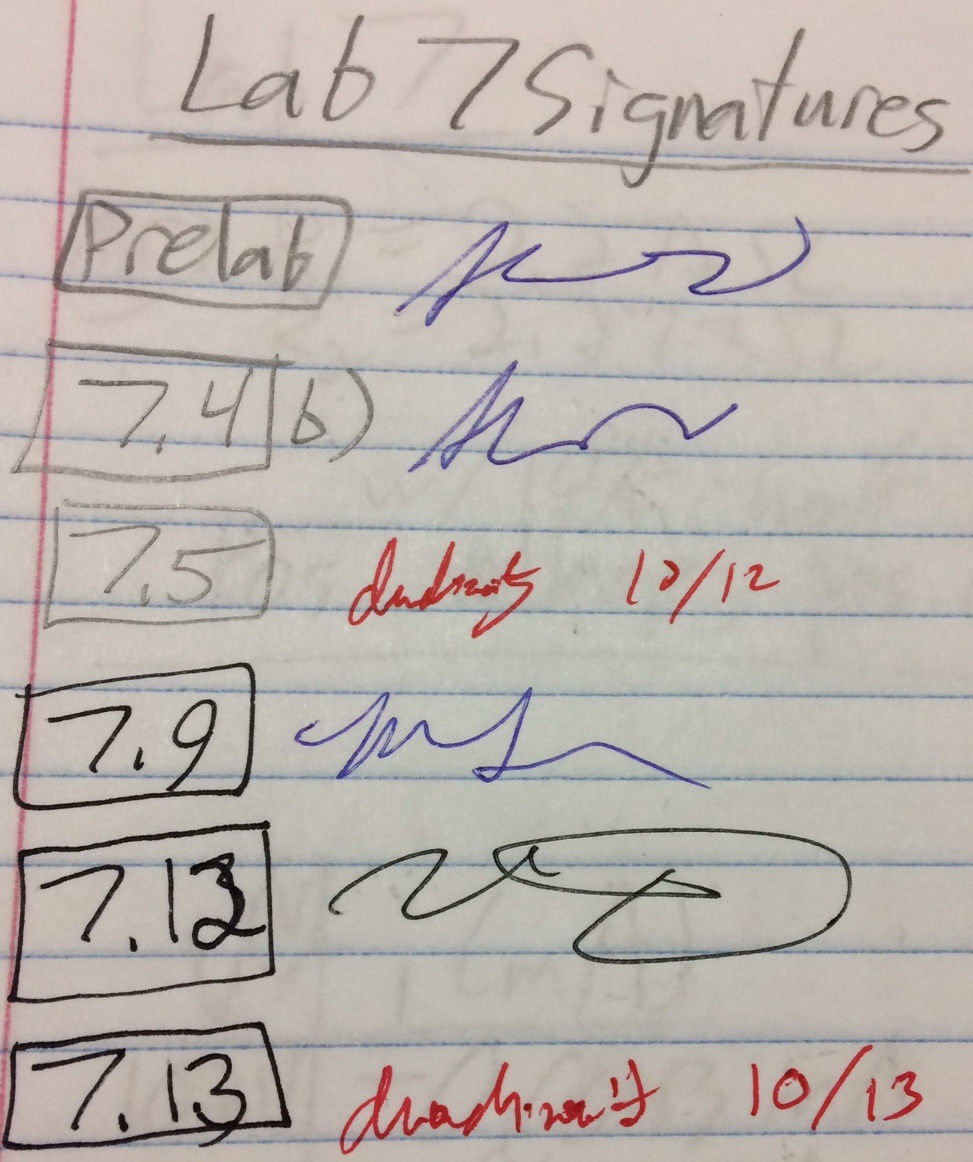
\includegraphics[scale = 0.3]{sig.JPG}
    \caption{Caption}
    \label{fig:my_label}
\end{figure}

\bibliography{joshbib}{}
\bibliographystyle{plain}

\end{document}

